\documentclass{article}
\usepackage[italian]{babel}
\usepackage[T1]{fontenc}
\usepackage{amsmath,amssymb,amsthm}
\usepackage{clrscode3e}

\usepackage{biblatex}
\addbibresource{./bibliography.bib}

\usepackage{enumerate}

\usepackage{epigraph}
\renewcommand{\epigraphrule}{0pt}
\renewcommand{\textflush}{flushepinormal}
\setlength{\epigraphwidth}{0.275\textwidth}
\renewenvironment{flushepinormal}{}{\vspace*{-\baselineskip}}

\usepackage{fontspec}
\usepackage{graphicx}
\usepackage{hyperref}
\usepackage{verbatim}

\graphicspath{ {./images/} }

\title{
  {
    \fontspec[ Path = fonts/ ]{Symbola}
    \symbol{"1F17C}\symbol{"1F435}\symbol{"1F17D}\symbol{"1F17A}ey
  } \large \\
  \small Relazione del progetto per l'insegnamento di Algoritmi e strutture di
  dati
}

\author{
  Gaia Clerici (\#971338),
  Stefano Volpe (\#969766)
}

\date{
	Universit\`a di Bologna \\
  \today
}

\begin{document}

\maketitle
\thispagestyle{empty}

\begin{figure}[h]
  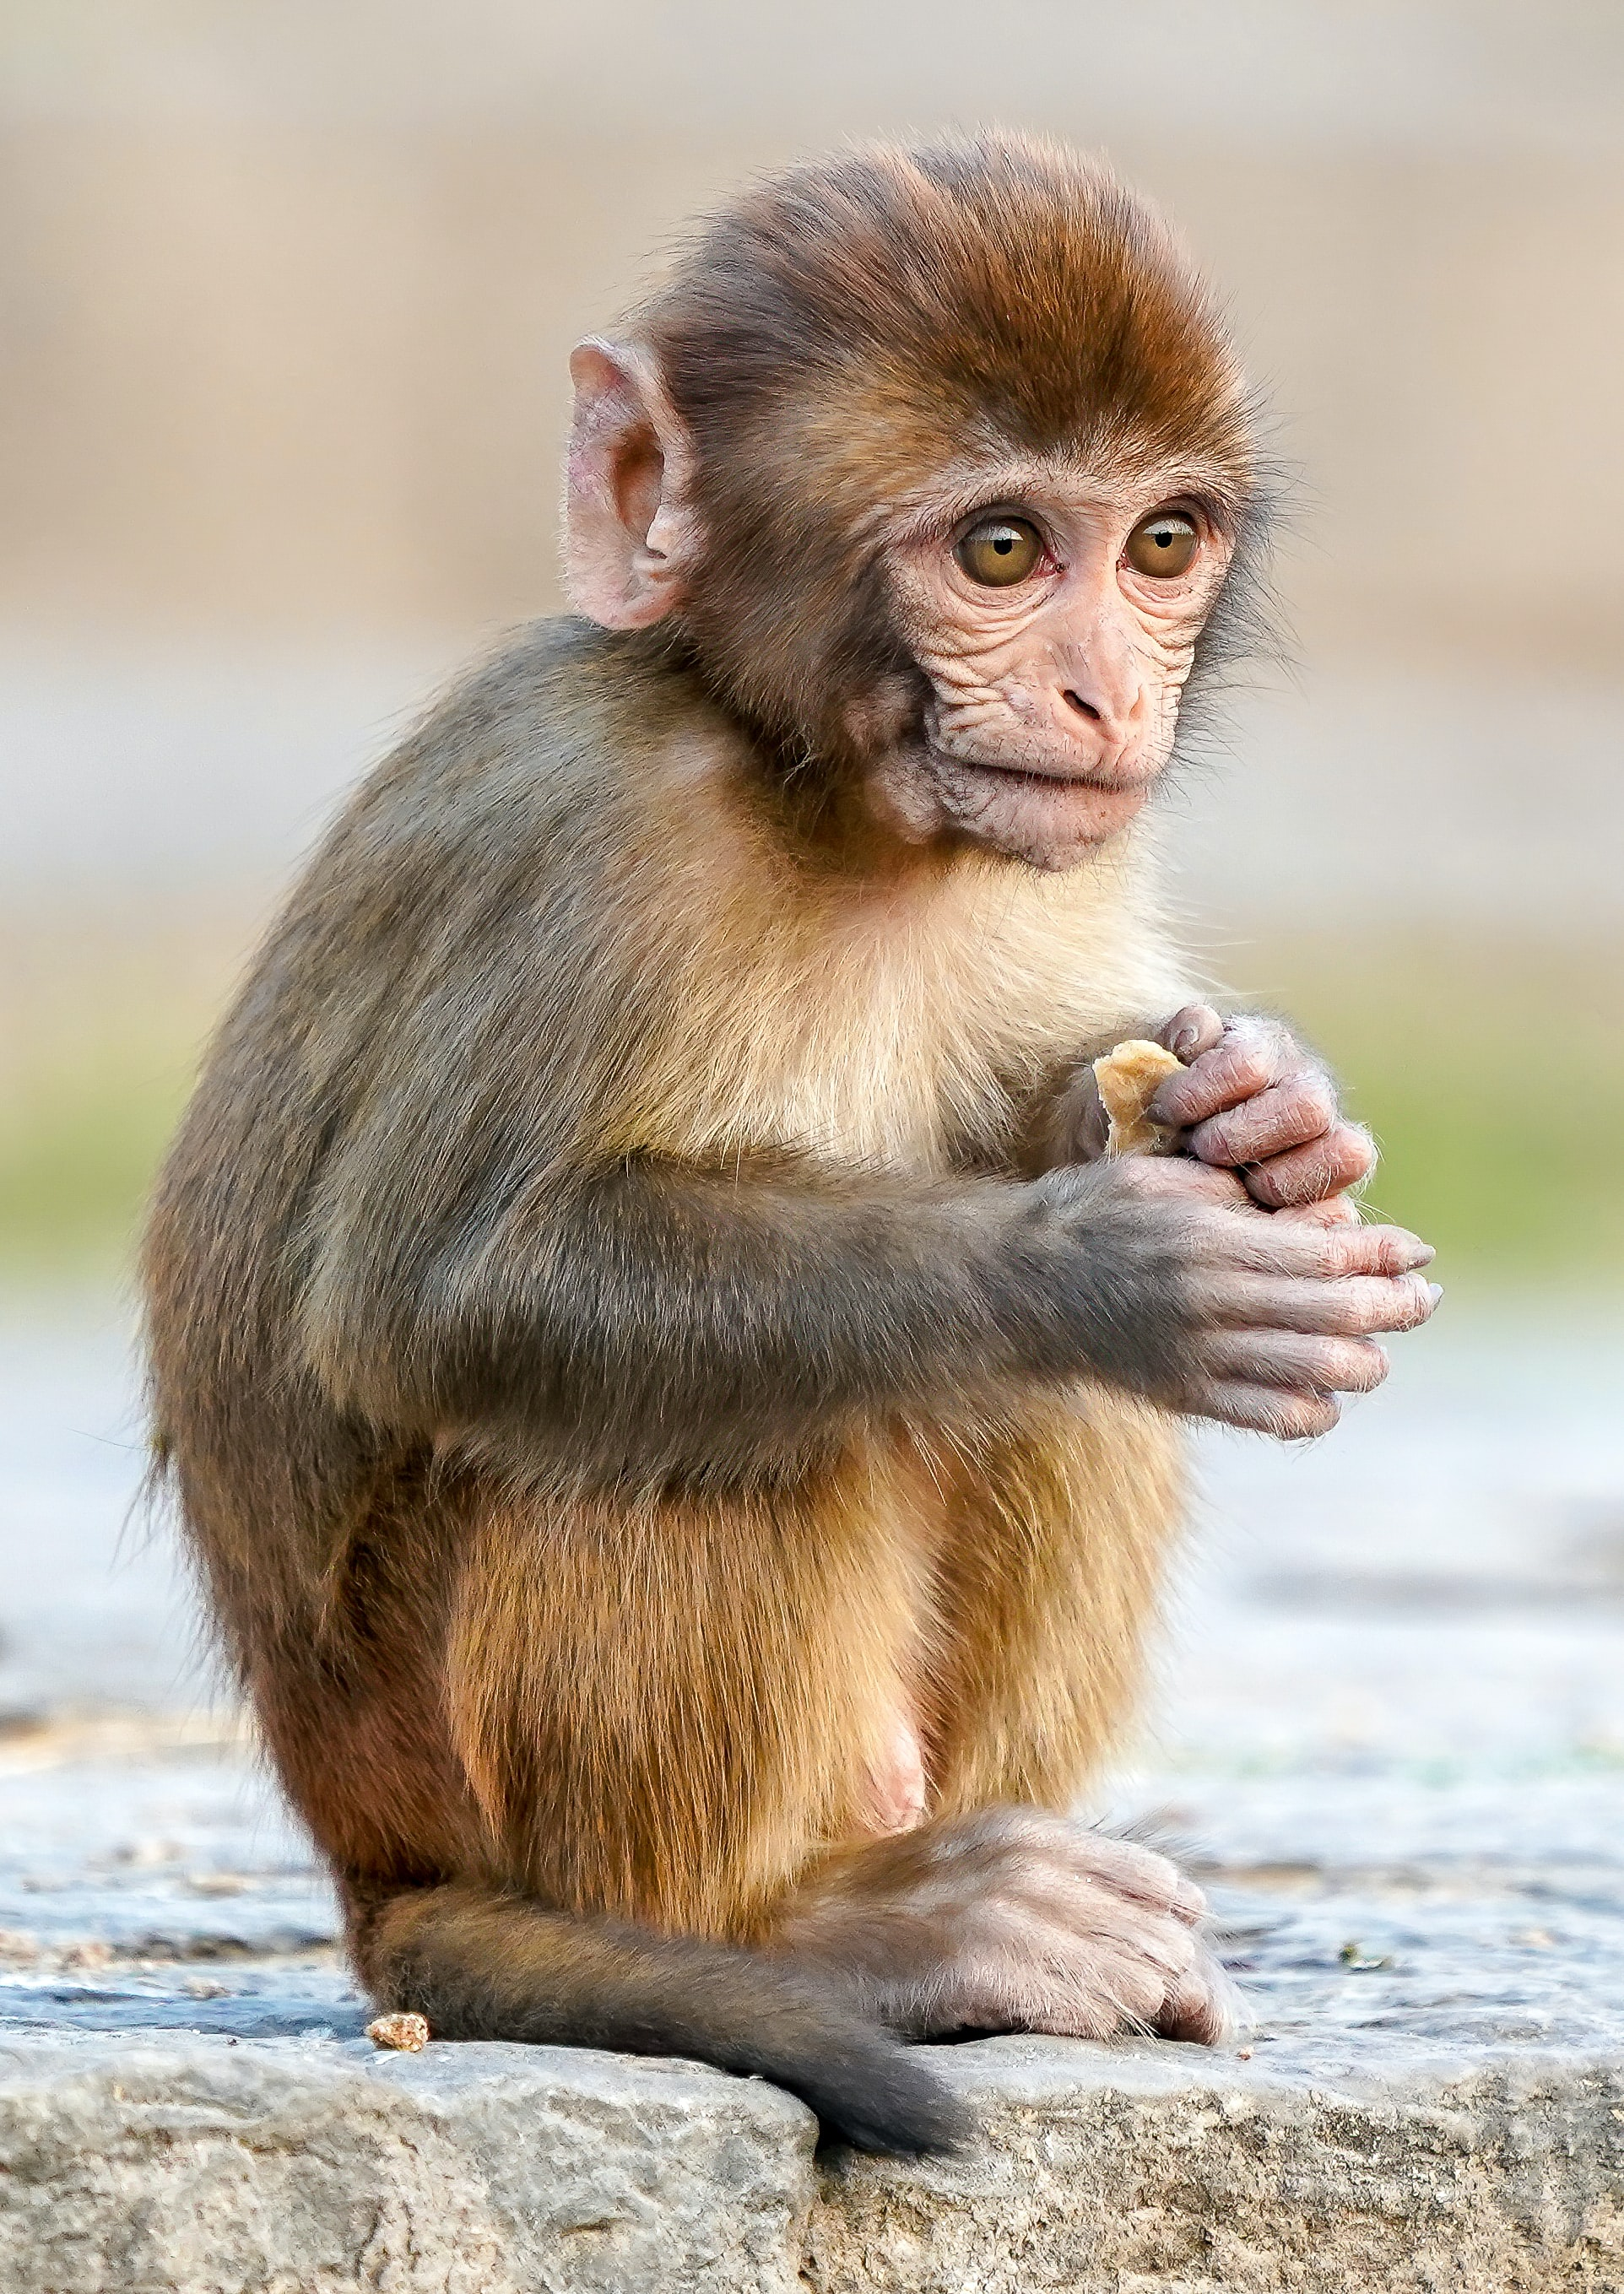
\includegraphics[width=0.75\textwidth]{monkey}
  \centering
  \caption{\href{https://unsplash.com/photos/daC7ji1EMHM}{una scimmia (foto di
  Bob Brewer)}}
\end{figure}

\pagebreak

\epigraph{Fa' la brava scimmietta.}{\textit{L'uomo con il cappello giallo}}

\tableofcontents

\pagebreak

\section{Specifiche}

\subsection{Il gioco: \emph{m,n,k-game}}

Il gioco \emph{m,n,k-game} è deterministico, a turni, a due giocatori, a somma
zero e con informazione perfetta. In una partita, i due agenti si alternano nel
marcare una cella vuota in una griglia di dimensione $m\times n$ con un simbolo
del proprio colore. Se un giocatore allinea in orizzontale, verticale o
diagonale almeno \emph{k} simboli, questi vince la partita e il suo avversario
la perde. Se non rimangono più celle vuote sulla griglia, la partita finisce
in pareggio.

\subsection{Il torneo: la classifica dei giocatori}

Ogni volta che, all'interno del torneo, un giocatore conclude una partita, egli
guadagna: 
\begin{itemize}
  \item 3 punti in caso di una vittoria come secondo giocatore, ma non a
    tavolino;
  \item 2 punti in caso di una vittoria come primo giocatore o a tavolino;
  \item 1 punto in caso di un pareggio;
  \item 0 punti in caso di una sconfitta.
\end{itemize}

\noindent
Le regole del torneo considerano una vittoria ``a tavolino'' quando l'avversario
non restituisce una mossa entro il tempo limite (approssimativo) di 10 secondi,
o comunque un mossa illegale (già occupata o esterna alla griglia). Non è dato
conoscere l'identità dell'avversario. Per ognuna delle seguenti configurazioni,
ciascun giocatore gioca esattamente quattro partite contro ogni altro
partecipante, di cui due come primo giocatore e due come secondo giocatore.

\begin{table}[h!]
\centering
\begin{tabular}{ | c | c | c | }
  \hline
  M & N & K \\
  \hline
  3 & 3 & 3 \\
  \hline
  4 & 3 & 3 \\
  \hline
  4 & 4 & 3 \\
  \hline
  4 & 4 & 4 \\
  \hline
  5 & 4 & 4 \\
  \hline
  5 & 5 & 4 \\
  \hline
  5 & 5 & 5 \\
  \hline
  6 & 4 & 4 \\
  \hline
  6 & 5 & 4 \\
  \hline
  6 & 6 & 4 \\
  \hline
  6 & 6 & 5 \\
  \hline
  6 & 6 & 6 \\
  \hline
  7 & 4 & 4 \\
  \hline
  7 & 5 & 4 \\
  \hline
  7 & 6 & 4 \\
  \hline
  7 & 7 & 4 \\
  \hline
  7 & 5 & 5 \\
  \hline
  7 & 6 & 5 \\
  \hline
  7 & 7 & 5 \\
  \hline
  7 & 7 & 6 \\
  \hline
  7 & 7 & 7 \\
  \hline
  8 & 8 & 4 \\
  \hline
  10 & 10 & 5 \\
  \hline
  50 & 50 & 10 \\
  \hline
  70 & 70 & 10 \\
  \hline
\end{tabular}
  \caption{configurazioni previste dal torneo.}
  \label{table:1}
\end{table}

\subsection{L'obiettivo: il giocatore}

Lo scopo del progetto è lo sviluppo di una intelligenza artificiale in Java
per il giocatore di \emph{m,n,k-game}. Se qualità della risposta e costo
temporale sono prioritari, lo stesso non vale per il costo in memoria, anche se
devono comunque essere evitati sprechi. Infine, a parità dei fattori di cui
sopra, la precedenza spetta alle strategie concettualmente più semplici.

\subsection{L'interfaccia: \texttt{mnkgame.MNKPlayer}}

L'interfaccia che l'intelligenza artificiale deve implementare è contenuta nel
pacchetto \verb!mnkgame!. Oltre a un metodo per la selezione della mossa
desiderata, ne viene concesso un altro invocato in fase di inizializzazione
prima di ogni partita.

\section{Analisi del problema}

\subsection{Il valore di gioco teorico}

Molte istanze del problema in questione si presentano come giochi a sé stanti,
talvolta arrichiti con limitazioni imposte dalle regole: ne sono esempi Tris,
Go-Moku e Renju. Per alcune configurazioni, il valore di gioco teorico è già
stato dimostrato. Herik, Uiterwijk e Rijswijck \cite{VANDENHERIK2002277} hanno
raccolto tali risultati dalla letteratura precedente nella seguente tabella.

\begin{table}[h!]
  \centering
  \begin{tabular}{ | c | c | c | }
    \hline
    mnk-game (k=1,2) & Vittoria per il primo giocatore \\
    \hline
    333-game (Tris) & Pareggio \\
    \hline
    mn3-game ($m \geq 4, n \geq 3$) & Vittoria per il primo giocatore \\
    \hline
    m44-game ($m \leq 8$) & Pareggio \\
    \hline
    mn4-game ($m \leq 5,n \leq 5$) & Pareggio \\
    \hline
    mn4-game ($m \geq 6,n \geq 5$) & Vittoria per il primo giocatore \\
    \hline
    mn5-game ($m \leq 6,n \leq 6$) & Pareggio \\
    \hline
    15,15,5-game (Go-Moku) & Vittoria per il primo giocatore \\
    \hline
    mnk-game ($k \geq 8$) & Pareggio \\
    \hline
  \end{tabular}
    \caption{valori di gioco di \emph{m,n,k-game}}
    \label{table:2}
  \end{table}

Tramite l'argomento del ``furto di strategia'', usato per la prima volta da John
Nash nel 1949 \cite{at.UBO716493520180101}, si dimostra che nessuno dei valori
di gioco teorico non ancora aggiunto alla tabella è una vittoria per il secondo
giocatore.

\subsection{L'albero di gioco}

Herik, Uiterwijk e Rijswijck \cite{VANDENHERIK2002277} classificano
\emph{m,n,k-game} come di ``categoria 3'', ovvero con un'alta complessità dello
spazio degli stati e una bassa complessità dell'albero di gioco. Per poter
quantificare meglio il numero di stati effettivamente appartenenti al nostro
albero di gioco, faremo uso del numero di celle della griglia come indice della
dimensione dell'istanza del problema. Esso vale:

\begin{equation}
s = m \times n
\end{equation}

Cominciamo osservando che il numero di figli $f$ di un qualsiasi nodo non
terminale a profondità $p$ coincide con il numero di celle rimaste vuote, e
cioè:

\begin{equation}
  f = s - p
\end{equation}

\section{Strumenti}

\section{Scelte progettuali}

Oltre a \verb!MoNKey.java!, che implementa \verb!mnkgame.MNKPlayer!, e
\verb!Tester.java!, classe di collaudo del progetto, \verb!monkey! disponde di
tre sottopacchetti:
\begin{itemize}
  \item \verb!monkey.util! fornisce strutture dati e algoritmi di uso generale
    ma non presenti nella libreria standard Java;
  \item \verb!monkey.ai! definisce un'intelligenza artificale per un generico
    gioco a turni a due giocatori i cui stati siano istanze di un'unica classe
    implementante \verb!monkey.ai.State!;
  \item \verb!monkey.mnk! espone la rappresentazione di \emph{m,n,k-game}
    implementando \verb!monkey.ai.State!.
\end{itemize}

\subsection{\texttt{monkey.util}}

\begin{sloppypar}
Questo pacchetto sopperisce alle mancanze della libreria standard con i metodi
per il calcolo del minimo e del massimo fra due elementi, nonché con una mappa
implementata come tabella ad indirizzamento diretto
\cite{at.UBO708344820100101}. Da notare che, fatta eccezione per
l'inizializzazione della suddetta mappa (che ha un costo temporale lineare nella
sua capacità), tutti i metodi di questo pacchetto hanno costo costante.
\end{sloppypar}

\subsection{\texttt{monkey.ai}}

L'intelligenza artificiale progettata propone due diversi algoritmi per la
scelta della mossa: il primo effettua una ricerca all'interno dell'albero di
gioco, mentre il secondo un più veloce ma meno accurato confronto fra le mosse
al momento disponibili. Quest'ultimo è pensato per le configurazioni troppo
impegnative per il primo algoritmo. Spetta a \verb!MoNKey.java! decidere a quale
metodo fare affidamento basandosi su $s$.

\subsubsection{Ricerca nell'albero di gioco}

Nonostante Herik, Uiterwijk e Rijswijck \cite{VANDENHERIK2002277} raccomandino
per i giochi di ``categoria 3'' l'uso di metodi basati sulla conoscenza,
abbiamo optato per una scelta più tradizionalista: una sintesi di più varianti
della potatura alfa-beta, che si colloca invece nei metodi a forza bruta.

In primo luogo, viste le imposizioni sul tempo di esecuzione, il nostro
algoritmo ha necessariamente bisogno di un limite di profondità $d$.
L'interfaccia delle due funzioni per una "classica" potatura alfa-beta risulta
quindi essere:
\begin{itemize}
  \item $\proc{Max-Value}(s, \alpha, \beta, d)$: applica la ricerca
    al nodo che rappresenta lo stato $s$ assumendo che esso sia di massimo;
  \item $\proc{Min-Value}(s, \alpha, \beta, d)$: applica la ricerca
    al nodo che rappresenta lo stato $s$ assumendo che esso sia di minimo.
\end{itemize}
In entrambi i casi, $\alpha$ e $\beta$ fungono da parametri della potatura,
mentre $d$ è il limite di profondità imposto. La mutuale ricorsione di queste
due procedure è responsabile di un'esplorazione a profondità limitata
dell'albero. La loro implementazione non viene riportata in quanto piuttosto
canonica, eccezion fatta per l'uso di una tabella delle trasposizioni.

\subsubsection{Confronto fra mosse}

\subsection{\texttt{monkey.mnk}}

\section{Conclusioni}

\section{Ricerche future}

\begin{sloppypar}
\printbibliography[
  heading=bibintoc
]
\end{sloppypar}

\end{document}
